\documentclass{amsart}
\usepackage{amsmath}
\usepackage{amssymb}
\usepackage{color}
\usepackage{tikz}
\usetikzlibrary{matrix,arrows,positioning,automata}
\usepackage{hyperref}
\definecolor{darkblue}{rgb}{0.0,0.0,0.3}
\definecolor{lgr}{rgb}{0.8,0.8,0.8}
\hypersetup{colorlinks,breaklinks,
            linkcolor=darkblue,urlcolor=darkblue,
            anchorcolor=darkblue,citecolor=darkblue}
\usepackage{wrapfig}

% NOTATION for diagram semigroups
\newcommand{\BinRel}{\text{B}}
\newcommand{\InvMon}{\mathcal I}
\newcommand{\DualInvMon}{{\mathcal I}^*}
\newcommand{\FullTrans}{\mathcal T}
\newcommand{\Symmetric}{\mathcal S}
\newcommand{\Brauer}{\mathfrak B}
\newcommand{\Partition}{\mathcal P}
\newcommand{\PartBinRel}{\Partition\BinRel}

\newcommand{\cD}{\mathcal D}



%\newcommand{\fJ}{\mathfrak J}



\newcommand{\todo}[1]{ \textsf{\color{red}{[TODO:  #1 ]}}}

\begin{document}
\section*{Representations of Finite Semigroups: Combinatorial Enumeration and Decomposition Methods}
%\section*{Representations of Finite Semigroups: Exploring the Land of Combinatorial Semigroups}

A \emph{transformation} is a function $f:X\rightarrow X$ from a set to itself.
In the finite case, this mathematical object is so basic, that we can easily answer all questions about it.
However, the situation changes dramatically when we start combining transformations.
A \emph{transformation semigroup} of degree $n$ is a collection of transformations of an $n$-element set closed under function composition.
\emph{How many degree $n$ transformation semigroups are there? ...up to conjugacy? ...up to isomorphism?}
These are typical combinatorial questions but an actual enumeration enables us to answer other type of important questions.
\emph{Can we represent a given abstract semigroup as transformations of $n$ points?}
\emph{What is the minimal value for such an $n$?}
In low-degree cases,  we can take the set of all transformations of $n$ points, the \emph{full transformation semigroup} $\FullTrans_n$, enumerate all of its subsemigroups, and by that we can find all possible degree-$n$ representations. 

\begin{wrapfigure}{R}{0.3\textwidth}
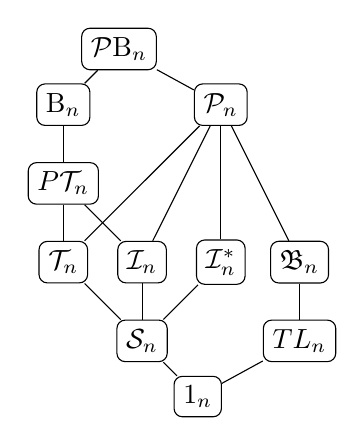
\begin{tikzpicture}
\tikzstyle{plain}=[rounded corners=3pt, draw]
\draw node [plain](Tn) {$\FullTrans_n$};
\draw node [plain,right of=Tn] (In) {$\InvMon_n$};
\draw node [plain,right of=In] (Ins) {$\DualInvMon_n$};
\draw node [plain,right of=Ins] (Br) {$\Brauer_n$};
\draw node [plain,below of=In] (Sn) {$\Symmetric_n$};

\draw node [plain,below right of=Sn] (1n) {$1_n$};
\draw node [plain,below of=Br] (TemperleyLieb) {$TL_n$};
\draw node [plain,above of=Tn] (PTn) {$P\FullTrans_n$};
\draw node [plain,above of=PTn] (Bin) {\BinRel$_n$};
\draw node [plain,above right of=Bin] (PBn) {$\PartBinRel_n$};
\draw node at (2,2) [plain] (PartitionMonoid) {$\Partition_n$};

\draw  (Tn) -- (Sn);
\draw  (In) -- (Sn);
\draw  (Ins) -- (Sn);

\draw  (PartitionMonoid) -- (In);
\draw  (PartitionMonoid) -- (Ins);
\draw  (PartitionMonoid) -- (Tn);
\draw  (PartitionMonoid) -- (Br);

\draw  (TemperleyLieb) -- (1n);
\draw  (Br) -- (TemperleyLieb);
\draw  (Sn) -- (1n);

\draw (PTn) -- (Tn);
\draw (PTn) -- (In);
\draw (Bin) -- (PTn);
\draw (PBn) -- (Bin);
\draw (PBn) -- (PartitionMonoid);
\end{tikzpicture}
\end{wrapfigure}
Previous efforts for enumerating semigroups were focused on the abstract case, enumerating by the order, and worked by finding all valid multiplication tables of the given size.
Here we plan to enumerate not by size but by a parameter of a given type of representation by finding all valid tables inside one big multiplication table of the corresponding full structure.
Since the multiplication table is representation independent, our method is not limited to transformation representations.
The whole combinatorial semigroup land (partial transformations and permutations, several diagram algebras contained in partition monoids), linear representations, and the practically important cascades  (tree transformations) can all be investigated by combinatorial enumeration methods.

Existing results also show that there are mind-blowing amount of semigroups even for low parameter values (52,989,400,714,478 abstract semigroups of order 9, XXX transformation semigroups on 4 points), and in this project we aim to tap into the vast stream of mathematical data produced by efficient enumeration algorithms in order to gain knowledge about representations far beyond the practically computable cases.
More precisely,
\begin{quote}
\noindent\emph{we aim to enumerate finite semigroups of different representations by multiplication table-based combinatorial algorithms, and by studying these low-degree cases we intend to formulate and prove theorems about representations of finite semigroups in general.}
\end{quote}


Generating  and validating this vast amount of data, compressing and making it accessible both computationally and mathematically  will require and provide new mathematical results.    

From the practical applications (biology, physics, artificial intelligence) point of view the cascade representations have utmost importance, since they are tightly connected to hierarchical decompositions, the algebraic ways of understanding complex systems. The biggest obstacle for these decomposition methods in realizing their potential is that we have limited understanding of the minimal tree transformation representations of semigroups. 

\begin{figure}
\begin{tabular}{|c|l|l|l|}
\hline
Symbol & Name &Order &$n=0,1,2,3,\ldots$\\ 
\hline 
$\PartBinRel_n$& \begin{minipage}[l]{130pt}Partitioned binary relations\end{minipage}  & $2^{(2n)^2}$ & $1, 16,65536,\ldots$\\
\hline 
$\BinRel_n$& \begin{minipage}[l]{130pt}Binary relations\end{minipage}  & $2^{n^2}$ & $1, 2, 16,512,65536,\ldots$\\
\hline 
$PT_n$& \begin{minipage}[l]{130pt}Full partial transformation semigroup\end{minipage}  & $(n+1)^n$ & $1, 2, 9, 64, 625, 7776,\ldots$\\
\hline 
$\Brauer_n$&Brauer monoid &$(2n-1)!!$ & $1, 1, 3, 15, 105, 945,\ldots$\\
\hline 
$\Symmetric_n$&symmetric group &$n!$ & $1, 1, 2, 6, 24, 120, 720,\ldots$\\
\hline 
$\FullTrans_n$&full transformation semigroup &$n^n$ & $1,1,4,27,256,3125,\ldots$\\
\hline
$\InvMon_n$&symmetric inverse monoid&$\sum_0^n k!{n\choose k}^2$ &$1, 2, 7, 34, 209, 1546,\ldots$\\
\hline
$\DualInvMon_n$&dual symmetric inverse monoid &$\sum_1^n k!\big(S(n, k)\big)^2$&$1, 1, 3, 25, 339, 6721,\ldots$\\
\hline
$TL_n,J_n$ & \begin{minipage}[l]{130pt}generators of Temperley-Lieb algebras, Jones monoid\end{minipage} & $C_n=\frac{1}{n+1} {2n \choose n}$ & $1,1,2,5,14,42, 132,\ldots$\\
\hline
\end{tabular}
\caption{Summary table of combinatorial semigroup representations. ($C_n$ is the $n$-th Catalan number, $S(n,k)$ are the Stirling numbers of the second kind)}
\end{figure}

\begin{enumerate}
\item Enumerate finite semigroups of different representations (across all types of diagrams) up to conjugacy and isomorphism.
\item Classify these semigroups according to their natural properties (size, ideal, $\cD$-class structure, etc.).
\item Study the results of the classification in order to establish new results for combinatorial representation theory of finite semigroups.
\item Study the properties of cascade representations in order to realize their application potential.
\end{enumerate}


\section{Diagram Semigroups}

For a $n$-element set $X$ a \emph{diagram} is a subset of $(X\cup X')\times (X\cup X')$ where $|X|=|X'|=n$ and $X\cap X'=\varnothing$.
In other words, a diagram is a relation on a set partitioned into two equal sized susbsets.
Pictorially we have an upper and lower set of points that may be connected by directed edges but with no parallel edges allowed.
Combining diagrams is stacking one on the top of the other and follow the arrows top-down and bottom-up, possibly removing combined paths that end or completely stay inside the middle. \todo{This isn't very precise, is it?}
The set of all diagrams of size $n$ form a monoid, $\Partition\BinRel_n$, the partitioned binary relations. 



\section{Sandbox}

Connections and allusions:
\begin{itemize}
\item Some of the diagram algebras have very sophisticated linear representation theories. Once we identify the the semigroups living in the diagrams, we have those representations for free. So semigroups act like the conduit for different results.
\end{itemize}

\end{document}
